\documentclass[14pt]{article}

\usepackage[utf8x]{inputenc}
\usepackage[russian]{babel}
\usepackage{graphicx}
\graphicspath{{images/}}
\DeclareGraphicsExtensions{.pdf,.png,.jpg}

\usepackage{amsmath}
\usepackage{pgfplots}

\usepackage{geometry} % Меняем поля страницы
\geometry{left=2cm}% левое поле
\geometry{right=1.5cm}% правое поле
\geometry{top=2cm}% верхнее поле
\geometry{bottom=2cm}% нижнее поле

\renewcommand{\theenumi}{\arabic{enumi}}% Меняем везде перечисления на цифра.цифра
\renewcommand{\labelenumi}{\arabic{enumi}}% Меняем везде перечисления на цифра.цифра
\renewcommand{\theenumii}{.\arabic{enumii}}% Меняем везде перечисления на цифра.цифра
\renewcommand{\labelenumii}{\arabic{enumi}.\arabic{enumii}.}% Меняем везде перечисления на цифра.цифра
\renewcommand{\theenumiii}{.\arabic{enumiii}}% Меняем везде перечисления на цифра.цифра
\renewcommand{\labelenumiii}{\arabic{enumi}.\arabic{enumii}.\arabic{enumiii}.}% Меняем везде перечисления на цифра.цифра

\begin{document}
\begin{titlepage}
	\begin{center}
		\fontsize{18pt}{20pt}\selectfont
		\textbf{Работа 1.4.5.}	
	
		\vspace{5cm}
		\fontsize{24pt}{25pt}\selectfont
		Изучение колебаний струны
	\end{center}
	\begin{flushright}
		\fontsize{18pt}{20pt}\selectfont
		\vspace{14cm}
		\hspace{-3cm}
		\textit{Корнеев Е.С.}
	\end{flushright}		
\end{titlepage}

\begin{center}
	\fontsize{16pt}{18pt}\selectfont	
	Изучение колебаний струны
\end{center}

\fontsize{14pt}{16pt}\selectfont
\vspace{1cm}
\textbf{Цель работы:} исследование зависимости частоты колебаний струны от величины натяжения, а также условий установления стоячей волны, получающейся в результате сложения волн, идущих в противоположных направлениях.

\vspace{0.5cm}
\textbf{В работе используются:} рейка со струной, звуковой генератор, постоянный магнит, разновесы.

\vspace{1cm}
%Основное свойство струны --- гибкость --- является следствием ее большой длины по сравнению с поперечными размерами.
Струной в акустике называют однородную тонкую гибкую упругую нить. Примерами могут служить сильно натянутый шнур или трос, струны гитары, скрипки и других музыкальных инструментов. В данной работе изучаются поперечные колебания стальной гитарной струны, натянутой горизонтально и закрепленной между двумя неподвижными зажимами.

Основное свойство струны --- гибкость --- обусловлено тем, что её поперечные размеры малы по сравнению с длиной. Это означает, что напряжение в струне может быть направлено только вдоль неё, и позволяет не учитывать изгибные напряжения, которые могли бы возникать при поперечных деформациях (то есть, при изгибе струны).

В натянутой струне возникает \textsl{поперечная упругость}, т.е. способность сопротивляться всякому изменению формы, происходящему без изменения обьема. При вертикальном смещении произвольного элемента струны, возникают силы, действующие на соседние элементы, и в резульатте вся струна приходит в движение в вертикальной плоскости, т.е. возбуждение «бежит» по струне. Передача возбуждения представляет собой поперечные бегущие волны, распространяющиеся с некоторой скоростью в обе стороны от места возбуждения. В ненатянутом состоянии струна не обладает свойством поперечной упругости и поперечные волны на ней невозможны.

\begin{figure}[h!]
	\center{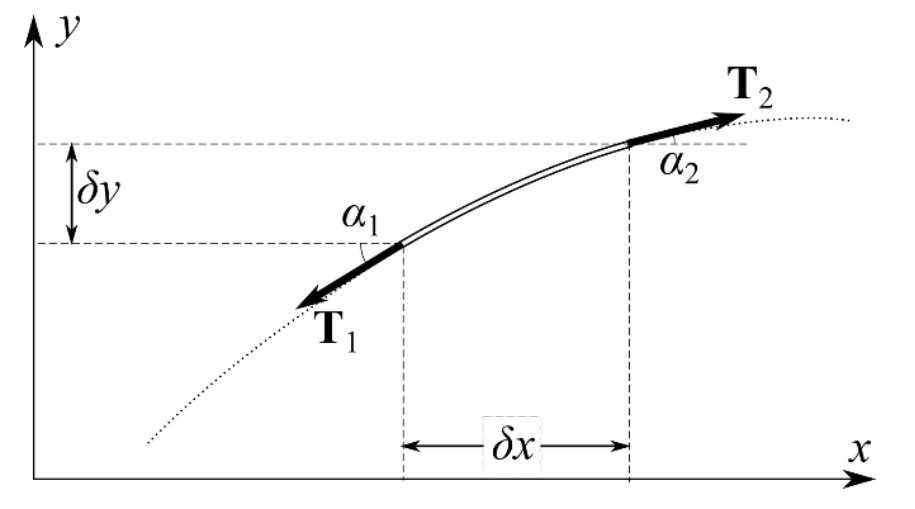
\includegraphics[width = 10cm]{im11}}
	\caption{К выводу уравнения колебаний}
	\label{fig:image}
\end{figure}

Рассмотрим гибкую однородную струну, в которой создано натяжение $T$, и получим дифференциальное уравнение, описывающее её малые поперечные свободные колебания. Отметим, что если струна расположена горизонтально в поле тяжести, величина $T$ должна быть достаточна для того, чтобы в
состоянии равновесия струна не провисала, т. е. сила натяжения должна существенно превышать вес струны.

Направим ось $x$ вдоль струны в положении равновесия. Форму струны будем описывать функцией $y(x, t)$, определяющей её вертикальное смещение в
точке $x$ в момент времени $t$ (рис. 1). Угол наклона касательной к струне в точке $x$ относительно горизонтального направления обозначим как 
$\alpha$. В любой момент этот угол совпадает с углом наклона касательной к графику функции $у(х)$, то есть 
$tg~a = \frac{\partial y}{\partial y}$.

Рассмотрим элементарный участок струны, находящийся в точке $x$, имеющий длину $\delta x$ и массу $\delta m = \rho \delta x$, где $\rho$ --- погонная плотность струны (масса на единицу длины). При отклонении от равновесия на выделенный элемент действуют силы натяжения $T_1$ и $T_2$, направленные по касательной к струне. Их вертикальная составляющая будет стремиться вернуть рассматриваемый участок струны к положению равновесия, придавая элементу некоторое вертикальное ускорение $\frac{\partial^2y}{\partial t^2}$. Заметим, что угол $\alpha$ зависит от координатs $x$ вдоль струны и различен в точках приложения сил $T_1$ и $T_2$. Таким образом, второй закон Ньютона для вертикального движения элемента струны запишется в следующем виде:

\begin{center}
\begin{equation}
\delta m \frac{\partial^2y}{\partial t^2} = -T_1\sin \alpha_1 + T_2\sin \alpha_2
\end{equation}
\end{center}


Основываясь на предположении, что отклонения струны от положения равновесия малы, можно сделать ряд упрощений:

1. Длина участка струны в изогнутом состоянии практически равна длине участка в положении равновесия, поэтому добавочным напряжением вследствие удлинения струны можно пренебречь. Следовательно, силы $T_1$ и $T_2$ по модулю равны силе натяжения струны: $T_1 \approx T_2 \approx T$.

2. Углы наклона $\alpha$ малы, поэтому $tg~\alpha \approx \sin\alpha \approx \alpha$ и, следовательно, можно положить $\alpha \approx \frac{\delta y}{\delta x}$.

Разделим обе части уравнения (1) на $\delta x$ и перейдем к дифференциалам:

\begin{center}
\begin{equation}
\rho \frac{\partial^2 y}{\partial t^2} = \frac{T_2\sin\alpha_2 - T_1\sin\alpha_1}{\delta x} = T\frac{\partial a}{\partial x}
\end{equation}
\end{center}

Подставим $\alpha = \frac{\partial y}{\partial x}$ и введем обозначение $u = \sqrt{\frac{T}{\rho}}$, что, как мы увидим далее, является скоростью распространения волн на струне, находим уравнение свободных малых поперечных колебаний струны:


\begin{center}
\begin{equation}
\boxed{\frac{\partial^2 y}{\partial t^2} = u^2 \frac{\partial^2 y}{\partial x^2}}
\end{equation}
\end{center}

Уравнение (3) называется \textsl{волновым уравнением}. Кроме волн на струне, оно может описывать волновые процессы в самых разных системах, в том числе волны в сплошных средах (звук), электромагнитные волныи т.д. 

\vspace{1cm}
\textbf{Бегущие волны}

Как показывается в математических курсах, общее решение дифференциального уравнения в частных производных (3) представимо в виде суммы двух волн произвольной формы, бегущих в противоположные стороны со скоростями $u$:

\begin{center}
\begin{equation}
y(x, t) = y_1(x - ut) + y_2(x + ut)
\end{equation}
\end{center}

\noindent где $u$ --- скорость распространения волны, $y_1$ и $y_2$ --- произвольные функции, вид которых определяется из начальных и граничных условий. При этом особый случай представляет случай гармонических волн:

\begin{center}
\begin{equation}
y(x, t) = a\cos[k(x - ut)] + b\cos[k(x + ut)] = a\cos(\omega t - kx) + b\cos(\omega t + kx)
\end{equation}
\end{center}

\noindent Выражение (5) представляет собой суперпозицию двух гармонических волн, бегущих навстречу друг другу со скоростью 

\begin{center}
\begin{equation}
u = \frac{\omega}{k} = \nu\lambda
\end{equation}
\end{center}

При этом длина волны $\lambda = \frac{2\pi}{k}$, частота $\nu = \frac{\omega}{2\pi}$. Величина $k = \frac{2\pi}{\lambda}$ называется \textsl{волновым числом} или \textsl{пространственной частотой волны}.

Заметим, что формула (2) означает, что скорость распространения волны зависит только от силы натяжения струны $T$ и погонной плотности $\rho$.

\vspace{1cm}
\textbf{Собственные колебания струны. Стоячие волны}

Найдем вид свободных колебаний струны с закрепленными концами. Пусть струна закреплена в точках $x = 0$ и $x = L$. Концы струны не колеблются, поэтому $y(0, t) = 0$ и $y(L, t) = 0$ для любых $t$. Используя (5), находим

$$y(0, t) = a\cos\omega t + b\cos\omega t = 0$$

\noindent откуда следует, что $a = -b$. Тогда после тригонометрических преобразований выражение (5) примет вид

\begin{center}
\begin{equation}
y(x, t) = 2a\sin kx \cdot \sin\omega t
\end{equation}
\end{center}

Колебания струны, описываемые функцией (7), называются \textsl{стоячими волнами}. Видно, что стоячая волна может быть получена как сумма (интерференция) двух гармонических бегущих волн, имеющих равную амплитуду и движущихся навстречу друг другу. Как видно из (7), точки струны, в которых $\sin kx = 0$, в любой момент времени неподвижны. Такие точки называются узлам. Остальные точки совершают в вертикальной плоскости гармонические колебания с частотой

$$\nu = \frac{\omega}{2\pi} = \frac{u}{\lambda}$$

Амплитуда колебаний распределена вдоль струны по гармоническому закону: $y_0(x) = 2a\sin kx$. В точках, где $\sin kx = 1$, амплитуда колебаний максимальна — они называются \textsl{пучностями}. Между двумя соседними узлами все участки струны колеблются в фазе (их скорости имеют одинаковое направление), а при переходе через узел фаза колебаний меняется на $\pi$ вследствие изменения знака $\sin kx$.

Используя второе граничное условие $y(L, t) = 0$ (точки крепления струны должны быть узлами стоячей волны), найдём условие образования стоячих
волн на струне: $y(x, t) = 2a\sin kL \sin \omega t = 0$, откуда 

$$\sin kL = 0 \Rightarrow kL = \frac{\pi}{2}n, n \in N$$

Таким образом, стоячие волны на струне с закреплёнными концами могут образовываться только если на длине струны укладывается целое число полуволн:

\begin{center}
\begin{equation}
L = \frac{\lambda}{2}n
\end{equation}
\end{center}

Поскольку длина волны однозначно связана с её частотой, струна может колебаться только с определёнными частотами:

\begin{center}
\begin{equation}
\nu_n = \frac{u}{\lambda_n} = \frac{n}{2L}\sqrt{\frac{T}{\rho}}, n \in N
\end{equation}
\end{center}

Набор (спектр) разрешённых частот $\nu_n$ называют \textsl{собственными частотами} колебаний струны. Режим колебаний, соответствующий каждой из частот $\nu_n$, называется собственной (или нормальной) \textsl{модой} колебаний (от англ. mode --- режим). Произвольное колебание струны может быть представлено в виде суперпозиции её собственных колебаний. Наименьшая частота $\nu_n$ называется также \textsl{основным тоном} (или первой гармоникой), а остальные ($\nu_2 = 2\nu_1$, $\nu_3 = 3\nu_1$, ...) --- \textsl{обертонами} (высшими гармониками). Термин «гармоника» иногда употребляется в обобщенном смысле — как элементарная составляющая сложного гармонического колебания.

На рис. 2 показана картина стоячих волн для $n = 1, 2, 3$. Заметим, что число $n$ определяет число пучностей (но не узлов!) колеблющейся струны. Таким образом, спектр собственных частот струны определён её погонной плотностью $\rho$, силой натяжения $T$ и длиной струны $L$ (отдельно отметим, что собственные частоты не зависят от модуля Юнга материала струны).

\begin{figure}[h!]
	\center{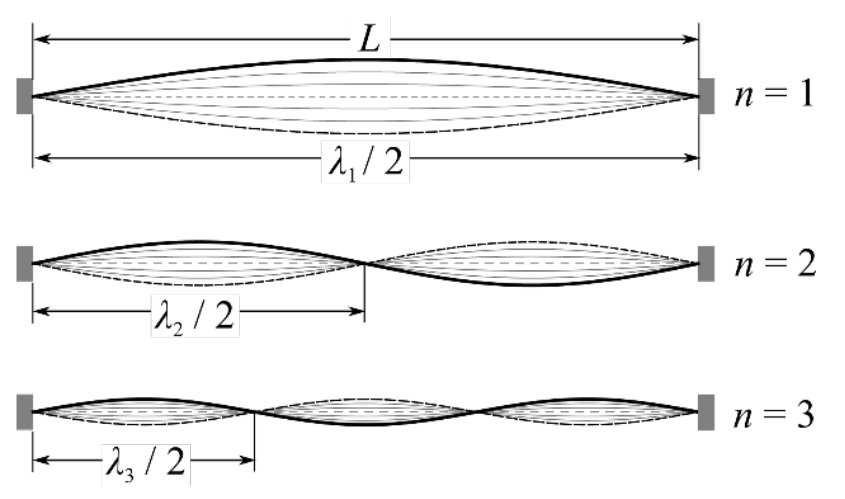
\includegraphics[width = 10cm]{im22}}
	\caption{Стоячие волны для $n = 1, 2, 3$}
	\label{fig:image}
\end{figure}

\vspace{1cm}
\textbf{Возбуждение колебаний струны}

При колебаниях реальной струны всегда имеет место потеря энергии (часть теряется вследствие трения о воздух; другая часть уходит через неидеально закрепленные концы струны и т.д.). Поддержание незатухающих колебаний в струне может осуществляться точечным источником, в качестве которого в данной работе используется электромагнитный вибратор. При этом возникает необходимость переноса энергии от источника по всей струне.

Рассмотрим вопрос о передаче энергии по струне. В стоячей волне поток энергии вдоль струны отсутствует — колебательная энергия, заключенная
в отрезке струны между двумя соседними узлами, не транспортируется в другие части струны. В каждом таком отрезке происходит периодическое (два-
жды за период) превращение кинетической энергии в потенциальную и обратно. Передача энергии между различными участками струны возможна только благодаря бегущим волнам, которые, однако, в рассмотренной выше идеальной модели струны не возникают. Парадокс снимается, если учесть, что из-за потерь энергии при отражении волны от концов не происходит полной компенсации падающей и отраженной волны, поэтому к стоячей волне на струне добавляется малая бегущая компонента — именно она служит «разносчиком» энергии по всей системе. 

Для эффективной раскачки колебаний используется явление резонанса --- вынуждающая частота $\nu$ должна совпадать с одной из собственных частот струны $\nu_n$ (9). Когда потери энергии в точности компенсируются энергией, поступающей от вибратора, колебания струны становятся стационарными и на ней можно наблюдать стоячие волны. Если потери энергии за период малы по сравнению с запасом колебательной энергии в струне, то искажение стоячих волн бегущей волной не существенно --- наложение бегущей волны малой амплитуды на стоячую визуально приводит к незначительному «размытию» узлов.

Для достижения максимального эффекта от вибратора, его следует располагать вблизи узловой точки. Это можно показать из следующих элементарных соображений. Пусть вибратор, размещённый в точке $x_0$, способен раскачать соответствующий элемент струны до амплитуды $A$. Если частота вибратора близка к резонансной (т.е. собственной), то как следует из (7), амплитуда колебаний струны в пучности будет равна 
$2a = \frac{A}{\sin kx_0}$. Таким образом, максимальная раскачка струны достигается, если значение $\sin kx_0$ устремить к нулю, что и соответствует положениям узлов (из идеализированной модели струны следует, что при размещении вибратора в узле амплитуда колебаний устремится к бесконечности, однако в реальности она ограничивается силами трения и нелинейными эффектами). Заметим также, что при наблюдении стоячих волн важно, чтобы колебания происходили в одной (вертикальной) плоскости, т.е. были поляризованы. Кроме того, важно, чтобы колебания струны происходили с малой амплитудой, поскольку при сильном возбуждении нарушаются условия применимости волнового уравнения (3), и в опыте наблюдаются искажения, связанные с нелинейными эффектами. 

\vspace{1cm}
\textbf{Экспериментальная установка}

Стальная гитарная струна закрепляется в горизонтальном положении между двумя стойками с зажимами, расположенными на массивной станине. Один конец струны закреплен в зажиме неподвижно. К противоположному концу струны, перекинутому через блок, прикреплена платформа с грузами, создающими натяжение струны. Зажим можно передвигать по станине, устанавливая требуемую длину струны. Возбуждение колебаний струны осуществляются с помощью электромагнитных датчиков (вибраторов), расположенных на станине под струной.

\begin{figure}[h!]
	\center{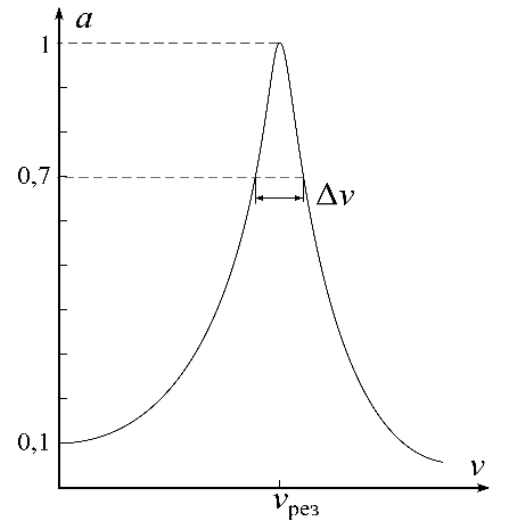
\includegraphics[width = 10cm]{im55}}
	\caption{АЧХ вынужденных колебаний}
	\label{fig:image}
\end{figure}

Дополнительным критерием того, что частота гармоники определена верно, является симметричность «резонансной кривой» — амплитудно-частотной характеристики системы. А именно, при подходе к резонансной частоте со стороны как высоких, так и со стороны низких частот, максимум сигнала наблюдается при одном и том же значении частоты.

\vspace{1cm}
\textbf{Нелинейные эффекты}

При сильном возбуждении струны нарушаются основные условия, при которых получено волновое уравнение (3). Возвращающая сила $T\sin\alpha$, действующая на элемент струны $\delta x$, в этом случае будет сама зависеть от величины $y$ --- отклонения элемента струны от положения равновесия. Кроме того, начинает играть существенную роль продольная деформация (растяжение) струны --- возникают добавочные напряжения, определяемые модулем Юнга материала струны. Поэтому форма резонансной кривой (АЧХ) струны начнет искажаться (рис. 4).

Каждый участок струны будет представим как нелинейный осциллятор. Как известно, частота собственных колебаний нелинейного осциллятора зависит от амплитуды. При умеренных амплитудах вынуждающей силы ($F_2$ на рис. 6) это приводит к смещению максимума резонансной кривой. Эффект смещения частоты тем сильнее, чем больше амплитуда колебаний струны. Вследствие этого, начиная с некоторого значения амплитуды силы ($F_3$ на рис. 6), резонансные кривые «опрокидываются» и приобретают неоднозначную «клювообразную» форму ($F_4$ на рис. 6). В таком случае в определённом интервале частот стационарная амплитуда вынужденных колебаний оказывается зависящей от предыстории установления колебаний --- возникает явление колебательного гистерезиса. При увеличении частоты (при подходе к резонансу «слева») амплитуда достигает максимума, после чего почти сразу происходит срыв колебаний (переход $A \rightarrow A'$), а при уменьшении частоты (подходе к резонансу «справа») возникает резкая раскачка колебаний на частоте, меньшей, чем резонансная (переход $B \rightarrow B'$). При этом на плоскости ($\nu, a$) образуется область физически нереализуемых режимов (закрашена серым).

\begin{figure}[h!]
	\center{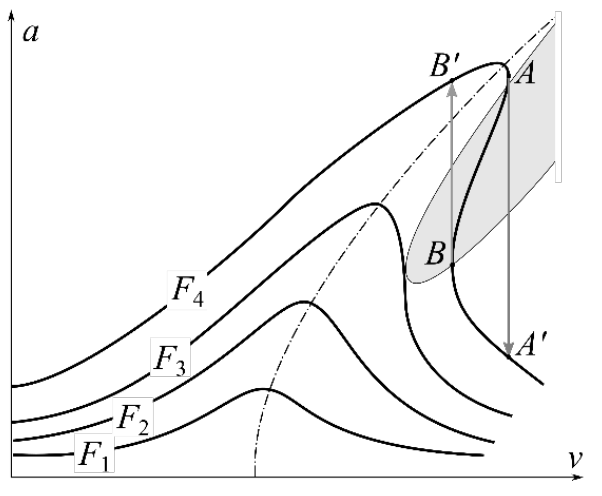
\includegraphics[width = 10cm]{im66}}
	\caption{АЧХ струны при $F_1 < F_2 < F_3 < F_4$}
	\label{fig:image}
\end{figure}

%%%%%%%%%
%
%	НАЧАЛО РАБОТЫ
%
%%%%%%%%%

\vspace{1cm}
\textbf{Визуальное наблюдение стоячих волн}

1. Освободим зажим струны на стойке 3, установим длину струны $L = 50$см. Натянем струну, поставив на платформу грузы ($F \approx 1$кг) (при этом учтем вес платформы и крепежа). Осторожно зажмем струну в стойке, не деформируя струну. Возбуждающий датчик 6 расположим рядом с неподвижной стойкой 2, т.е. вблизи узла стоячей волны. 

2. Проведем предварительные расчёты. Оценим скорость распространения волн по формуле (2), используя табличное значение плотности стали и приняв диаметр струны равным $d \approx 0.3$мм. Для заданных значений длины струны и силы натяжения рассчитаем частоту основной гармоники $\nu_1$ согласно (9).

3. Включим в сеть звуковой генератор и частотомер. Установим на генераторе тип сигнала --- синусоидальный, частоту основной гармоники $\nu_1$ и максимальную амплитуду напряжения. При этом сигнал с выхода генератора должен быть подан на возбуждающий датчик 6.

4. Медленно меняя частоту звукового генератора в диапазоне $\nu = \nu_1 \pm 5$Гц, добьемся возбуждения стоячей волны на основной гармонике (одна пучность). Определим частоту первой гармоники по частотомеру. 

5. Увеличив частоту в 2 раза, получим картину стоячих волн на второй гармонике, а затем и на более высоких гармониках. Запишем значения частот $\nu_n$ стоячих волн, которые удастся пронаблюдать.


6. Проведем опыты для пяти различных натяжений струны. При изменении нагрузки ослабим зажим струны в стойке 3, положим груз на чашку и вновь осторожно зажмем струну.

\vspace{1cm}
\textbf{Обработка результатов измерений}

1. По результатам измерений построим графики зависимостей частоты $\nu_n$ от номера $n$ гармоники для различных натяжений $T$. Определим скорости волн $u$, бегущих по струне. Оценим погрешность измерения $u$.

2. Построим график зависимости квадрата скорости $u^2$ от силы натяжения $T$. Определим погонную плотность струны $\rho$ и оценим погрешность результата. Сравним полученное значение $\rho$ со значением погонной плотности струны, указанной на установке.

\vspace{1cm}
Построим таблицу зависимости частоты $\nu$ от массы подвеса $m$. Здесь $m$ - сумма масс грузика и подвеса ($m_\text{подв} = 25$г):

\begin{center}
\begin{tabular}{|c|c|c|c|c|c|c|c|c|c|c|c|c|c|c|c|c|c|}
\hline
\multicolumn{3}{|c|}{$m = 75$г}&\multicolumn{3}{|c|}{$m = 65г$}&\multicolumn{3}{|c|}{$m = 55$г}&\multicolumn{3}{|c|}{$m = 35$г}&\multicolumn{3}{|c|}{$m = 90$г}\\
\hline
$n$	&$\nu$, Гц	&$\delta\nu$&$n$ &$\nu$, Гц&$\delta\nu$&	$n$	&$\nu$, Гц &$\delta\nu$&$n$	&$\nu$, Гц&$\delta\nu$&	$n$	&$\nu$, Гц&$\delta\nu$\\
\hline
1	&51.2		&5			& 1	  &48.9	  	&10		  	&	1	&45.0		&4		  	&1	&38.6	  &7	  	  &	1	&58.7		&8			\\
\hline
2	&101.0		&10			& 2	  &96.3		&8		  	&	2	&82.3		&8		  	&2	&73.7	  &10	  	  &	2	&114.1		&7			\\
\hline
3	&155.1		&8			& 3   &			&		  	&	3	&125.6		&8		  	&3	&110.0	  &10	  	  &	3	&169.3		&6			\\
\hline
4	&210.6		&6			& 4	  &191.4	&10		  	&	4	&169.2		&6		  	&4	&		  &		  	  &	4	&226.0		&4			\\
\hline
5	&262.1		&4			& 5	  &240.9	&6		  	&	5	&213.8		&5		  	&5	&183.7	  &8	  	  &	5	&			&			\\
\hline
6	&311.0		&4			& 6   &287.1	&4		  	&	6	&258.3		&6		  	&6	&220.2	  &7	  	  &	6	&			&			\\
\hline
7	&361.6		&5			& 7   &			&		  	&	7	&			&			&7	&		  &	  	  	  &	7	&			&			\\
\hline
\end{tabular}
\end{center}

Построим графики $\nu_n$ от $n$ для различных масс:

\vspace{1cm}
\hspace{2cm}$m = 75$г
\begin{flushleft}
\begin{tikzpicture}
\begin{axis}[
	height = 9cm,
	width  = 14cm,
	every axis y label/.style={at = {(ticklabel cs: 0.5)}, rotate = 90, anchor = near ticklabel},
	xlabel = {$n$},
	ylabel = {$\nu_n$, Hz}
]
\addplot+[smooth, error bars/.cd, 
	y dir = both, y explicit,
	x dir = both, x explicit,
	] 
coordinates{
	(1,  51.2) +- (0, 5)
	(2, 101.0) +- (0, 10)
	(3, 155.1) +- (0, 8)
	(4, 210.6) +- (0, 6)
	(5, 262.1) +- (0, 4)
	(6, 311.0) +- (0, 4)
	(7, 361.6) +- (0, 4)
};
\end{axis}
\end{tikzpicture}
\end{flushleft}

\vspace{2cm}
\hspace{2cm}$m = 65$г
\begin{flushleft}
\begin{tikzpicture}
\begin{axis}[
	height = 9cm,
	width  = 14cm,
	every axis y label/.style={at = {(ticklabel cs: 0.5)}, rotate = 90, anchor = near ticklabel},
	xlabel = {$n$},
	ylabel = {$\nu_n$, Hz}
]
\addplot+[smooth, error bars/.cd, 
	y dir = both, y explicit,
	x dir = both, x explicit,
	] 
coordinates{
	(1,  48.9) +- (0, 10)
	(2,  96.3) +- (0, 8)
	(4, 191.4) +- (0, 10)
	(5, 240.9) +- (0, 6)
	(6, 287.1) +- (0, 4)
};
\end{axis}
\end{tikzpicture}
\end{flushleft}

\vspace{1cm}
\hspace{2cm}$m = 55$г
\begin{flushleft}
\begin{tikzpicture}
\begin{axis}[
	height = 9cm,
	width  = 14cm,
	every axis y label/.style={at = {(ticklabel cs: 0.5)}, rotate = 90, anchor = near ticklabel},
	xlabel = {$n$},
	ylabel = {$\nu_n$, Hz}
]
\addplot+[smooth, error bars/.cd, 
	y dir = both, y explicit,
	x dir = both, x explicit,
	] 
coordinates{
	(1,  46.0) +- (0, 4)
	(2,  82.3) +- (0, 8)
	(3, 125.6) +- (0, 8)
	(4, 169.2) +- (0, 6)
	(5, 213.8) +- (0, 5)
	(6, 258.3) +- (0, 6)
};
\end{axis}
\end{tikzpicture}
\end{flushleft}

\vspace{4cm}
\hspace{2cm}$m = 35$г
\begin{flushleft}
\begin{tikzpicture}
\begin{axis}[
	height = 9cm,
	width  = 14cm,
	every axis y label/.style={at = {(ticklabel cs: 0.5)}, rotate = 90, anchor = near ticklabel},
	xlabel = {$n$},
	ylabel = {$\nu_n$, Hz}
]
\addplot+[smooth, error bars/.cd, 
	y dir = both, y explicit,
	x dir = both, x explicit,
	] 
coordinates{
	(1,  38.6) +- (0, 7)
	(2,  74.0) +- (0, 10)
	(3, 110.0) +- (0, 10)
	(5, 183.0) +- (0, 8)
	(6, 220.0) +- (0, 7)
};
\end{axis}
\end{tikzpicture}
\end{flushleft}

\vspace{1cm}
\hspace{2cm}$m = 90$г
\begin{flushleft}
\begin{tikzpicture}
\begin{axis}[
	height = 9cm,
	width  = 14cm,
	every axis y label/.style={at = {(ticklabel cs: 0.5)}, rotate = 90, anchor = near ticklabel},
	xlabel = {$n$},
	ylabel = {$\nu_n$, Hz}
]
\addplot+[smooth, error bars/.cd, 
	y dir = both, y explicit,
	x dir = both, x explicit,
	] 
coordinates{
	(1,  58.0) +- (0, 8)
	(2, 114.4) +- (0, 7)
	(3, 170.0) +- (0, 6)
	(4, 228.0) +- (0, 4)
};
\end{axis}
\end{tikzpicture}
\end{flushleft}


\vspace{1cm}
Зная, что $u = \frac{2\nu_nL}{n}$, найдем $u$ для различных значений силы натяжения. $\nu_n/n$ найдем из угловых коэффициентов графиков для соответствующих масс. $2L$ для всех случаев одинакова и равна $2\cdot 0.5 = 1$м.

\begin{center}
\begin{tabular}{|c|c|c|c|c|c|c|c|c|c|c|c|c|c|c|}
\hline
$k_{max}$, Гц&	$k_{min}$, Гц&	$k$, Гц	&$\Delta k$, Гц	&$T$, Н		&$u$, м/с&$\Delta u$, м/с&$u^2, \text{м}^2/c^2$&$\Delta u^2,\text{м}^2/c^2$\\
\hline
52.4		&	50.8		&	51.6	&	0.8			&	0.74	&51.6	 &	0.8			  	&	2662.6			&	82.5	\\
\hline
48.5		&	47.2		&	47.9	&	0.7			&	0.64	&47.9	 &	0.7				&	2294.4			&	64.4	\\
\hline
45.0		&	42.0		&	43.0	&	1.0			&	0.54	&44.0	 &	1.0				&	1849.0			&	86.0	\\
\hline
37.7		&	35.5		&	36.6	&	1.1			&	0.34	&36.6	 &	1.1				&	1339.6			&	80.5	\\
\hline
58.6		&	56.0		&	57.6	&	1.0			&	0.88	&56.6	 &	1.0				&	3203.6			&	114.0	\\
\hline
\end{tabular}
\end{center}


\vspace{1cm}
Построим график зависимости $u^2(T)$:

\vspace{1cm}
\begin{flushleft}
\begin{tikzpicture}
\begin{axis}[
	height = 9cm,
	width  = 14cm,
	every axis y label/.style={at = {(ticklabel cs: 0.5)}, rotate = 90, anchor = near ticklabel},
	xlabel = {$T, H$},
	ylabel = {$u^2, m^2/c^2$}
]

\addplot+[error bars/.cd, 
	y dir = both, y explicit,
	x dir = both, x explicit,
	] 
coordinates{
	(0.34, 1340) +- (0, 80)
	(0.54, 1950) +- (0, 86)
	(0.64, 2294) +- (0, 64)
	(0.74, 2662) +- (0, 83)
	(0.88, 3200) +- (0, 114)
};
\end{axis}
\end{tikzpicture}
\end{flushleft}

\vspace{1cm}
Из графика: $\rho = T/u^2$.

$$\rho_{min} = 2.67, \text{мг/см}$$
$$\rho_{min} = 2.84, \text{мг/см}$$

Отсюда:

$$\boxed{\boxed{\rho_{min} = (2.76 \pm 0.08) \text{мг/см}}}$$

\newpage
Таким образом, в данной лабораторной работе мы изучили колебания струны и поведение стоячих волн. Особо стоит отметить тот факт, что при больших амплитудах действительно наблюдались <<срывы>>, а также то, что некоторые моды так и не удалось достичь. Также интересным оказалось явление, при котором число пучностей было в два раза меньше, чем ожидалось, причем это состояние струна принимала всегда при данных значениях силы натяжения и возбуждающей частоты.

\newpage
Список использованной литературы:
	
\vspace{0.5cm}
1. "Лабораторный практикум по общей физике: Учебное пособие. В трех томах. Т1. Механика"/А.Д.Гладун, Д.А.Александров,
Ф.Ф.Игошин и др.; Под редакцией А.Д.Гладуна. --- МФТИ, 2004.
	
2. "Набор и верстка в системе \LaTeX "/С.М.Львовский. --- 2003.






\vspace{1cm}
\hspace{2cm}$m = 75$г
\begin{flushleft}
\begin{tikzpicture}
\begin{axis}[
	height = 9cm,
	width  = 14cm,
	every axis y label/.style={at = {(ticklabel cs: 0.5)}, rotate = 90, anchor = near ticklabel},
	xlabel = {$n$},
	ylabel = {$\nu_n$, Hz}
]
\addplot+[smooth, error bars/.cd, 
	y dir = both, y explicit,
	x dir = both, x explicit,
	] 
coordinates{
	(1,  51.2) +- (0, 5)
	(2, 101.0) +- (0, 10)
	(3, 155.1) +- (0, 8)
	(4, 210.6) +- (0, 6)
	(5, 262.1) +- (0, 4)
	(6, 311.0) +- (0, 4)
	(7, 361.6) +- (0, 4)
};
\addplot+[smooth, error bars/.cd, 
	y dir = both, y explicit,
	x dir = both, x explicit,
	] 
coordinates{
	(1,  48.9) +- (0, 10)
	(2,  96.3) +- (0, 8)
	(4, 191.4) +- (0, 10)
	(5, 240.9) +- (0, 6)
	(6, 287.1) +- (0, 4)
};
\addplot+[smooth, error bars/.cd, 
	y dir = both, y explicit,
	x dir = both, x explicit,
	] 
coordinates{
	(1,  46.0) +- (0, 4)
	(2,  82.3) +- (0, 8)
	(3, 125.6) +- (0, 8)
	(4, 169.2) +- (0, 6)
	(5, 213.8) +- (0, 5)
	(6, 258.3) +- (0, 6)
};
\addplot+[smooth, error bars/.cd, 
	y dir = both, y explicit,
	x dir = both, x explicit,
	] 
coordinates{
	(1,  38.6) +- (0, 7)
	(2,  74.0) +- (0, 10)
	(3, 110.0) +- (0, 10)
	(5, 183.0) +- (0, 8)
	(6, 220.0) +- (0, 7)
};
\addplot+[smooth, error bars/.cd, 
	y dir = both, y explicit,
	x dir = both, x explicit,
	] 
coordinates{
	(1,  58.0) +- (0, 8)
	(2, 114.4) +- (0, 7)
	(3, 170.0) +- (0, 6)
	(4, 228.0) +- (0, 4)
};
\end{axis}
\end{tikzpicture}
\end{flushleft}







\end{document}